\section{Overall description}

\subsection{General product description}
\writer{Marius - Anders - Georgios}

This section contains a description of the software, as well as the actors identified and details on
how the final system works. 

Petri nets are a mathematical modeling language which is used for describing the operational flow of
systems with dynamic and discrete behavior. Some examples of domains in which Petri nets have a
clear applicability are material flow, transportation or distributed computing. However, this
modeling language misses two critical characteristics that would have made it even more useful.
Petri Nets do not provide a domain-specific visualization, being therefore challenging even for the
most experienced users when trying to understand the full operational flow of a complex system based
only on the original graphical notation. Moreover, Petri nets are discrete, implying that systems
that indicate a continuous behavior are challenging to be modeled.

Some of these extension might deserve a brief presentation.
In figure \ref{fig:petri-semaphore} a semaphore is shown.
The dottet circle represents an input place.
Input places are places where extra tokens can be placed from an external source,
in this case when a user clicks an object in the simulator.
In figure \ref{fig:petri-semaphore} the semaphore is green.
Tracks are places with a special identifier, in this example track places are colored red
as well as the arcs connecting them.
Whenever a ``train token'' appears on the left track place $L$, the transition $S$ will fire.
The token in the semaphore will be consumed by $T$ and produced again.
The train token will be produced in $R$.
\begin{figure}[htp]
\begin{center}
\begin{petri}[Very][Simple]
    \node at (2, 5) [place] (red) {};
    \node at (2, 2) [place] (green) {};
	\node at (-0.5, 0) [track place] (left track) {$L$};
	\node at (4.5, 0) [track place] (right track) {$R$};
    \node at (2, 3.5) [inputplace] (input) {$I$};
	\node at (0.5, 3.5) [transition] (turn green) {$T_G$};
	\node at (3.5, 3.5) [transition] (turn red) {$T_R$};
	\node at (2, 0) [transition] (connection) {$S$};
	\node at (2, 2) [token] {};
	\draw [->,arc] (red) to [out=180,in=90] (turn green);
	\draw [->,arc] (green) to [out=0,in=270] (turn red);
	\draw [->,arc] (turn green) to [out=270,in=180] (green);
	\draw [->,arc] (turn red) to [out=90,in=0] (red);
	\draw [->,arc] (input) to [out=0,in=180] (turn red);
	\draw [->,arc] (input) to [out=180,in=0] (turn green);
	
	\draw [->,arc] (connection) to [out=75,in=285] (green);
	\draw [->,arc] (green) to [out=255,in=105] (connection);
	\draw [->,track arc] (left track) -- (connection);
	\draw [->,track arc] (connection) -- (right track);
\end{petri}
\caption{Petri net for a semaphore}
\label{fig:petri-semaphore}
\end{center}
\end{figure}
If anybody clicks the object representing the semaphore in the simulator,
a token will be placed in $I$, and the $T_R$ (Turn Red) transition will fire.
Both the new token in $I$ and the token in the lower semaphore place will be consumed.
A new token will produced in the upper semaphore place.
$S$ will not be able to fire in this state of the Petri net - the semaphore is red.

The next example in figure \ref{fig:petri-switch} illustrates a switch $I$ will change the switch state.
As it is on the example the train token will choose the lower track.
But it will wait until its animation is finished.
The token is not marked as ready, illustrated by red filling (marked tokens are filled black).
When the animation, probably one moving the traing from one end of the track to the other, is finished,
the token will be marked (turn black) and the transition $T$ can fire.

\begin{figure}
\begin{center}
\begin{petri}
	\node at (2, 5) [place] (left) {};
	\node at (2, 2) [place] (right) {};
	\node at (2, 3.5) [inputplace] (input) {$I$};
	\node at (0.5, 3.5) [transition] (turn right) {};
	\node at (3.5, 3.5) [transition] (turn left) {};
	\node at (2, 0) [transition] (go right) {$T$};
	\node at (2, 7) [transition] (go left) {};
	\node at (-2, 3.5) [track place] (incoming track) {};
	\node at (2, 2) [token] {};
	\node at (-2, 3.5) [train token] {};
	\draw [->,arc] (left) to [out=180,in=90] (turn right);
	\draw [->,arc] (right) to [out=0,in=270] (turn left);
	\draw [->,arc] (turn right) to [out=270,in=180] (right);
	\draw [->,arc] (turn left) to [out=90,in=0] (left);
	\draw [->,arc] (input) to [out=0,in=180] (turn left);
	\draw [->,arc] (input) to [out=180,in=0] (turn right);
	
	\draw [->,arc] (go right) to [out=75,in=285] (right);
	\draw [->,arc] (right) to [out=255,in=105] (go right);

	\draw [->,arc] (go left) to [out=255,in=105] (left);
	\draw [->,arc] (left) to [out=75,in=285] (go left);

	\draw [->,track arc] (incoming track) to [out=30,in=180] (go left);
	\draw [->,track arc] (incoming track) to [out=-30,in=180] (go right);
	\draw [->,track arc] (go right) -- (4,0);
	\draw [->,track arc] (go left) -- (4,7);
	\draw [->,track arc] (-4,3.5) -- (incoming track);
\end{petri}
\caption{Petri net for a switch}
\label{fig:petri-switch}
\end{center}
\end{figure}


As a basis for our subsequent explanations and descriptions, we consider the Petri net example in
Figure \ref{fig:petrinet_example}. It is a Petri net which models a railway with three signals, one
switch and a train. The places, transitions and tokens are based on the ones in a classic Petri net.

\begin{figure}[htp]
    \begin{center}
		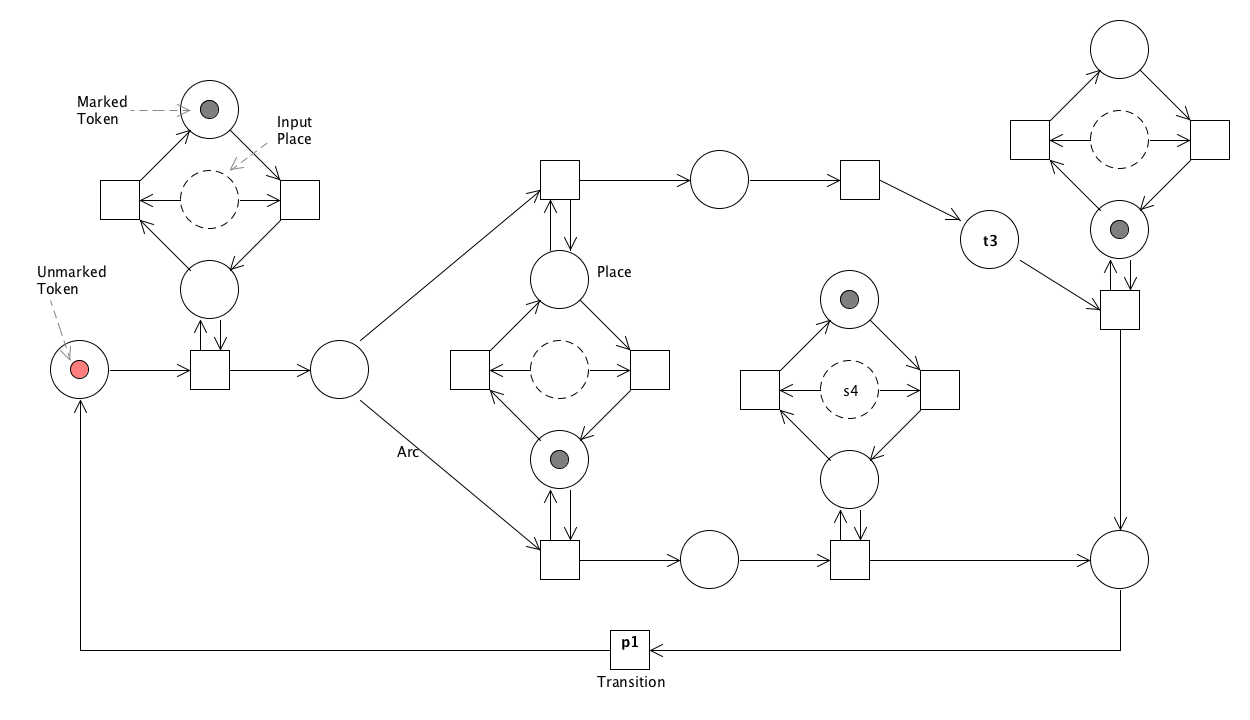
\includegraphics[scale=0.35]{image/petrinet_example.png}
		\caption{Petri net example}
		\label{fig:petrinet_example}
	\end{center}
\end{figure}

For the purpose of creating a 3D visualization of systems that can be modelled as a Petri net, the
application's user has to configure where the objects should be represented in the 3D space (and
this is what we called ''geometry'') and what the objects look like (''appearance''). Continuing our
example of the railway, for a proper visualization, the shape of the track has to be defined and the
positions of other elements (e.g. signals, switches) have to be fixed. An example of such a
configuration can be seen in Figure \ref{fig:geometry_example}.

\begin{figure}[htp]
	\begin{center}
		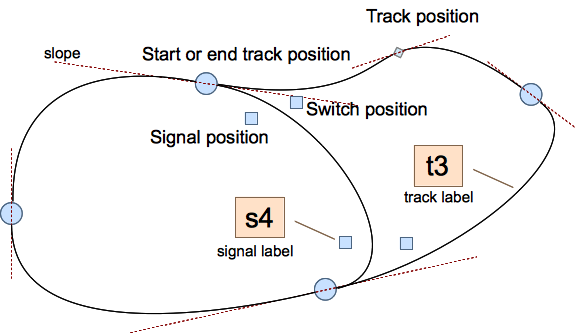
\includegraphics[scale=0.40]{image/geometry_example.png}
		\caption{Geometry example}
		\label{fig:geometry_example}
	\end{center}
\end{figure}

The ultimate goal of \epns is to visualize and interact with a dynamic system by using an
extended Petri net model enriched with features that will allow the user to correlate the model with
the physical world. Animation and visualization of an underlying Petri net model would constitute an
excellent feature that could potentially assist users in efficiently examining and analyzing the
model.

The following actors have been identified:

\begin{description}
    \item[the technical user] - has knowledge of Petri nets and uses the software
    to design the networks according to the desired specifications.
	\item[the non-technical user] -doesn't know the specifics of Petri nets, but needs to see the
	simulation of a discrete system, so he can have a better understanding of the real-life system.
	This type of user will only use pre-existing Petri nets (could be Petri nets created by the first
	type of user), with the required additional configurations, and run the simulation.
\end{description}

The following case is used to prove the utility of the project in a practical scenario. An engineer
could use this tool to design the extended Petri net, assigning any possible attributes to it (such
as shape and identity), so as to include any possible characteristics of the physical 3D objects he
might want to visualize. After the completion of the Petri net configuration, this technical user
could couple the underlying model with a 3D-animation to present it to his manager. The manager does
not need to have any understanding of Petri nets, but he can still evaluate the model and get a
clear view of its internal functionality.

From the user's point of view, the system can be divided in three parts:

\begin{description}
	\item[the Petri net and Animation Editor] - where a user (the technical user)
	sets the design of the Petri net, the animation associated with each place and
	the appearance of a token.
	\item[the Geometry Editor] - where a (technical) user sets the geometry of the
	system; for the railway example, in the geometry editor, the user sets the
	shape, length and appearance of the railway.
	\item[the Simulator] - where both types of users can see a 3D representation
	of the modeled system.
\end{description}

All the components and the way they interact with one another will be thoroughly described in the
following sections.

\subsection{Basic functionality}
\writer{Cosmin}
In order to use \epns, the application user starts by using the \textbf{Petri net Editor} to create
and configure the Petri net and the \textbf{Animations} that are executed during the simulation.
These will be later loaded by the \textbf{Graphical Simulator}, which, after being started, will
simulate the movement of tokens through the Petri net and will execute the configured animations,
resulting a visual representation of the Petri net's simulation on the screen.

Then, using the \textbf{GeometryEditor}, the \textbf{Geometry} would be created. It would be later
used by the \textbf{Graphical Simulator} in order to know how (on which paths) to move objects/token
representations and where to place different objects in the 3D space\footnote{Even though the
geometry is specified in a 2D space, during the simulation, all the object representations will be
drawn as 3D objects moving on a plane.}.

The \textbf{Graphical Simulator} also requires information about the \textbf{Appearance}, in order
to know how to represent tokens, tracks and other objects during the simulation. It is a simple
editor that connects labels (keys) with 3D Models(vrml, png, jpg \ldots), textures or just plain
data (Colors, Shapes).
  
The last step is to create a \textbf{Configurator} that connects the previously created
configurations and allows the user to start the graphical simulation. When started, the
\textbf{Graphical Simulator} reads the state of the simulation from the \textit{Petri net}. This read
state does not include exact positions of tokens in space, this information being loaded from the
\textit{Geometry}, or appearance information, loaded from the \textit{Appearance}. After
initialization, the Graphical Simulator displays the state of the simulation and handles all the
users' interaction as specified in the rest of this document.

For further details of what exactly each of the components allows the users to do please check the
following section or, in order to get more details regarding how to use \epns, please read the
\textit{Handbook}.

\subsection{General concepts}
\writer{Cosmin}
\label{oa:generalconcepts}
This subsection will introduce the general concepts used in the \epns system. More details will be
provided in the~\nameref{sec:architecture} and~\nameref{sec:system_features} sections, however the
most important concepts are presented below.

First of all, the classical concepts of \textbf{Petri nets} have been extended to accommodate the
required information for the graphical visualization of the simulation:
\index{Petri net} 
\begin{description}
\index{Petri net!Input Place}
\item[Input Places] - in order to provide the users with more power and customizability, some of the
Places in the Petri net can be configured to allow users, during the graphical simulation, to drop
(create) tokens. These are called \textit{Input Places} and act as normal Places in all other
respects, except for that they permit the possibility of a token being created there. For example,
in a train track simmulation, it allows the creation of simulation features such as a Traffic lights
or switches with which the users can interact during the graphical simulation.
\index{animation}
\item[Animations] - can be associated by the user to a particular Place and are run when a Token is
added on that Place, either by result of executing a transition or by being dropped there (after a
user interaction). Even though the token is removed from the source Places of the fired Transition,
they are not available for firing a new Transition until the animations associated with a place are
finished. More details will be specified later, but the supported animation types include: moving an
object on a path, showing or hiding objects, wait a fixed amount of time.
\item[Place Appearance] - each Place can have an associated appearance, describing how it must look
like in the Graphical Simulator.
\item[Token Appearance] - each Token can have an associated appearance, describing how it must look
like in the Graphical Simulator. Thus, the appearance of a Token will not change based on a place.
This will allow multiple tokens, with different representations, to be on the same place/track.
\item[Arc Identities] - each arc can have attached an identity used to control the flow of tokens
(or, more precisely, of token representations) in the simulation. For e.g., if we have a Transition
with one input Arc and two output Arcs and we take the case of simulating a train running on a
track, using the same identity on the input Arc and on one of the ouput Arcs will tell the Graphical
Simulator to move the Token representation (a train), which came on the input Arc, on the
corresponding output Arc. This allows a token representation to move continously in the direction
the user wants, without being destroyed or unnecessarily recreated.
\end{description}

Regarding the \textbf{Geometry}, as defined, it allow the users to specify the positions of objects
and the paths on which they move in the simulation space. The most important related concepts that
need to be presented at this point are:
\index{geometry}
\begin{description}
\index{Petri net!Track}
\item[Track] - defines how a curve (or line), on which an animation can take place, looks like. It
can also be connected with information about what the surface of this track looks like and usually
are used as graphical representations of Places.
\index{Petri net!Simple Position}
\item[Simple Position] - defines just a position in the simulation space and can be connected to the
an appearance it has. Can be used for completing the specification of some animations, for
representing an Input Place or just for displaying simple objects during the simulation.
\end{description}

Referring to the \textbf{Appearance}, it allow the users to easily define how objects look like
during the simulation. In \epns, there are mainly two big types of appearances that can be
configured:
\index{appearance}
\begin{description}
\item[Shape] - defines how a 3D Object displayed in the simulation should look like. For example, it
can be a reference to a file storing a 3D Model, which can then be loaded in the application or it
can simply be a 3D Object, such as a Cube or Sphere.
\item[Surface] - defines how a surface displayed in the simulation should look like. It can be
applied, for example, to a train track, and it could be either just a Color or a reference to a file
containing a texture that can be applied on the surface.
\end{description}


